\documentclass[10pt,a4paper]{article}
\usepackage[utf8]{inputenc}
\usepackage[german]{babel}
\usepackage[T1]{fontenc}
\usepackage{amsmath}
\usepackage{amsfonts}
\usepackage{amssymb}
\usepackage{graphicx}
\renewcommand\thesubsection{\alph{subsection}}
\begin{document}

\begin{center}
\begin{LARGE}
Praktikum 1\\
Differentialgleichungen
\end{LARGE}
\end{center}

\section{Lösung  "`steifer Differentialgleichungen"' mit Euler/Runge-Kutta (RK 2. Ordng.)}

\subsection{Geben Sie das Analogrechner-/Simulink-Schaltbild an.}
\begin{figure}[h]
\centering
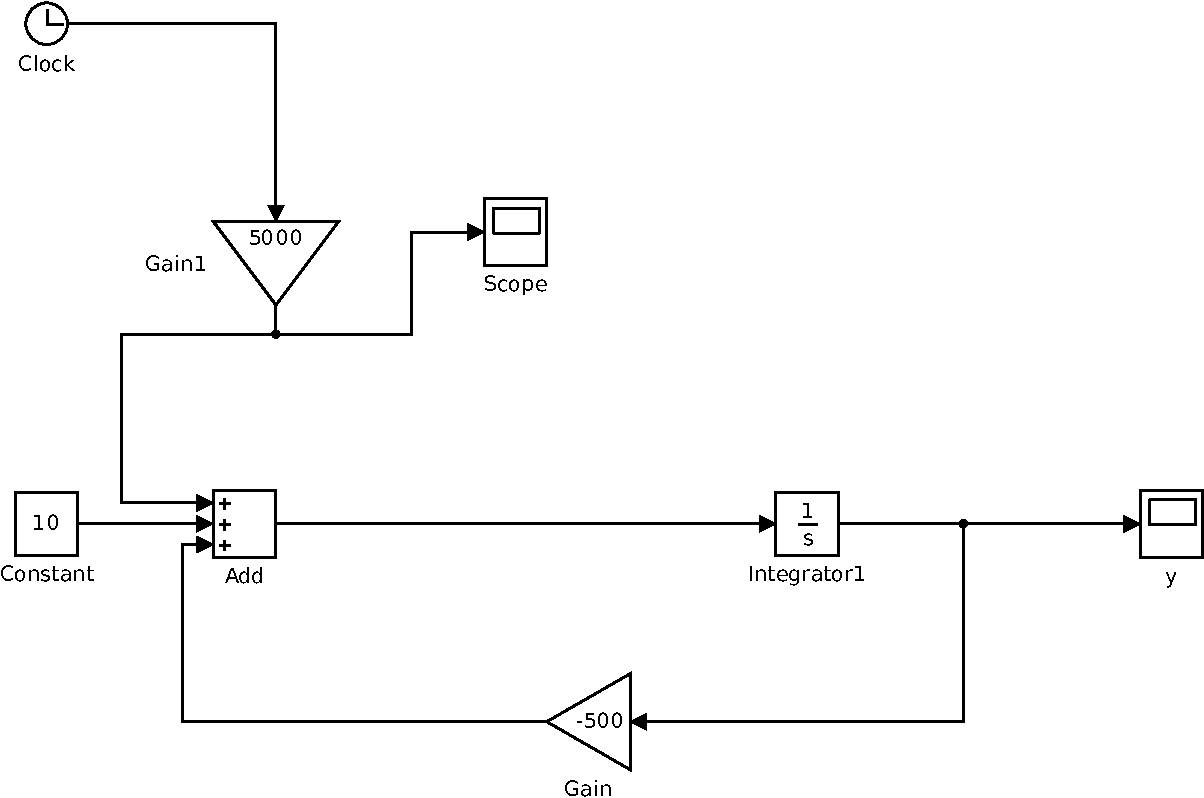
\includegraphics[width=0.9\linewidth]{../screenshots/1}
\end{figure}
\subsection{Geben Sie die Iterationsgleichungen für das Euler-Verfahren an.}
\subsection{Geben Sie die Iterationsgleichungen für das RK2-Verfahren an.}
\subsection{Geben Sie die Iterationsgleichungen für das implizite Euler-Verfahren an.}
\subsection{Schreiben Sie ein Programm "`Stiff.ch"', welches die DGL mit allen Verfahren
löst und zusammen mit der analytischen Lösung in einem Plot anzeigt.}

\begin{center}
\begin{large}
Versuchsdurchführung
\end{large}
\end{center}


\section{Lösung einer (nichtlinearen) DGL 2. Ordnung (Van-der-Pol-DGL) mit RK 2}
\subsection{Geben Sie das Analogrechner-/Simulink-Schaltbild an.}
\begin{figure}[h]
\centering
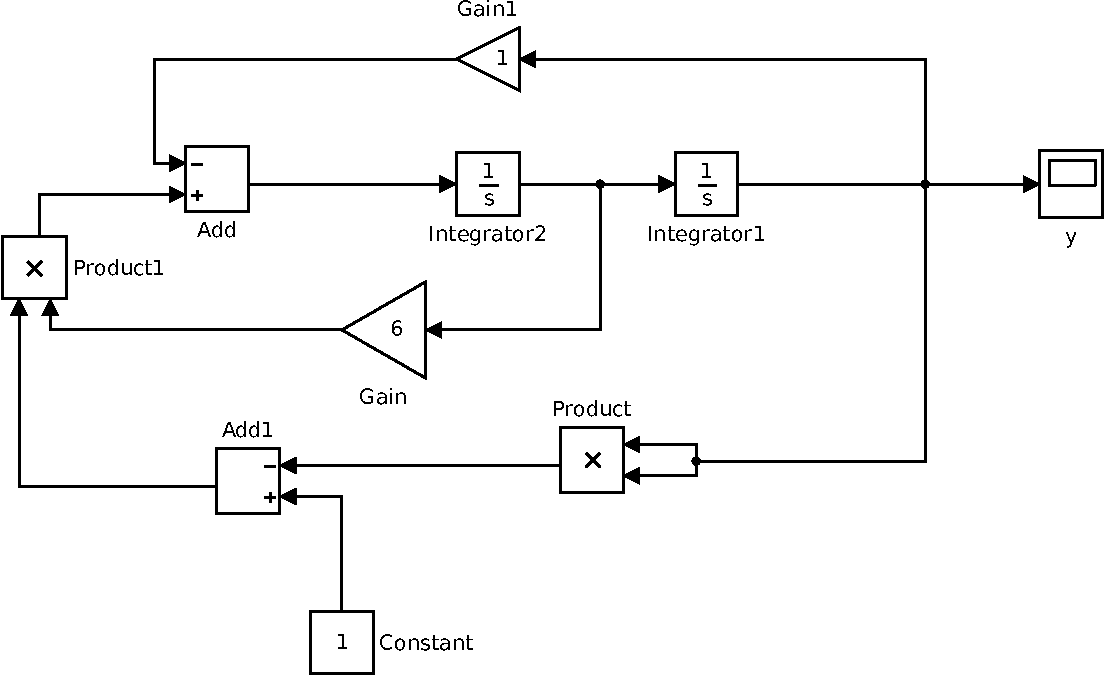
\includegraphics[width=0.9\linewidth]{../screenshots/2}
\end{figure}
\subsection{Geben Sie die DGL 2. Ordnung als 2 DGLn 1. Ordnung an.}
\subsection{Geben Sie die Iterationsgleichungen für das Euler-Verfahren an.}
\subsection{Geben Sie die Iterationsgleichungen für das RK2-Verfahren an.}
\subsection{Schreiben Sie ein Programm "VanDerPol.ch", welches die DGL mit beiden
Verfahren löst und in einem Plot anzeigt.}

\begin{center}
\begin{large}
Versuchsdurchführung
\end{large}
\end{center}

\section{Lösung eines Differentialgleichungssystems (Lorenz-Attraktor) mit RK 2}
\subsection{Geben Sie die Iterationsgleichungen für das RK2-Verfahren an.}
\subsection{Schreiben Sie ein Programm "Lorenz.ch", welches das DGL-System löst.
Geben Sie im 1. Plot die Funktion x(t) aus:
Geben Sie im 2. Plot z(x) aus.}
\subsection{Realisieren Sie das Differentialgleichungssystem mit MATLab/Simulink}
\begin{figure}[h]
\centering
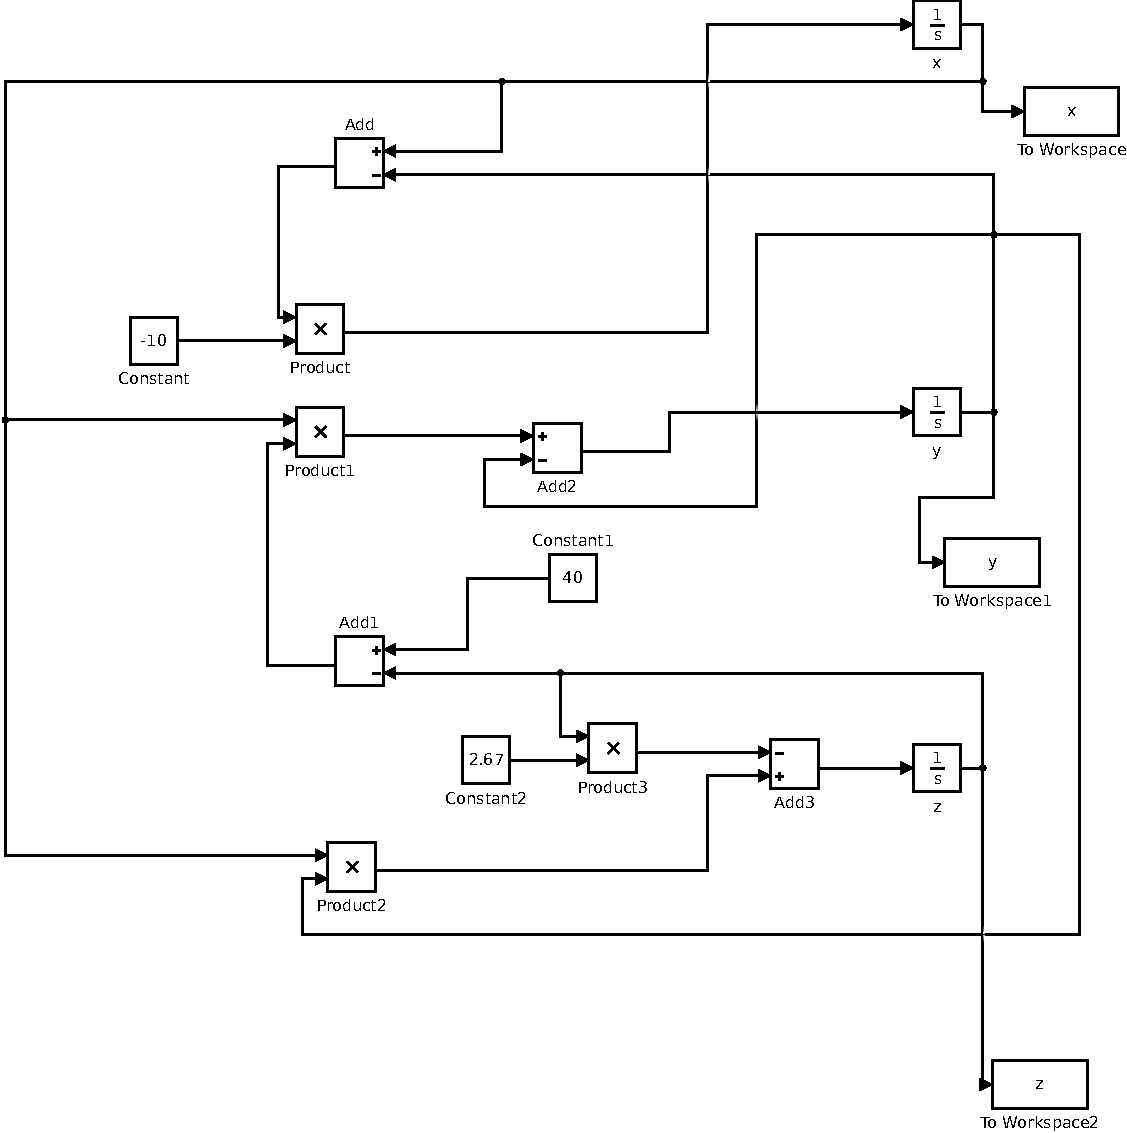
\includegraphics[width=0.9\linewidth]{../screenshots/3}
\end{figure}

\begin{center}
\begin{large}
Versuchsdurchführung
\end{large}
\end{center}

\end{document}